\subsubsection{2.2. Tiền xử lý dữ liệu}

\textit{2.2.1. Xây dựng đặc trưng nút}\vspace{0.2cm}

\indent Để tạo ra biểu diễn toàn diện cho mỗi thực thể trong mạng lưới, đề tài thực hiện tổng hợp biểu diễn ngữ nghĩa văn bản và các chỉ số hành vi định lượng, thiết lập một không gian đặc trưng hỗn hợp phục vụ mục tiêu phân loại Sybil.\vspace{0.3cm}

Quá trình bắt đầu bằng việc xây dựng dữ liệu định danh từ các trường \texttt{handle}, \texttt{display\_name} và \texttt{bio}, được ghép nối theo cấu trúc: \texttt{"Handle: \{h\}. Name: \{n\}. Bio: \{b\}"}. Bằng cách giữ nguyên ngữ cảnh tự nhiên và các ký tự đặc biệt, đề tài sử dụng mô hình \textbf{all-MiniLM-L6-v2} để ánh xạ chuỗi văn bản thành vector ngữ nghĩa \textbf{384 chiều}.\vspace{0.3cm}

Song song đó, 12 chỉ số hành vi định lượng — bao gồm cường độ tương tác nội dung, điểm tin cậy trên nền tảng và thời gian hoạt động — được trích xuất để mô tả đặc tính của nút. Các giá trị thiếu (\textit{NULL}) được mặc định gán bằng \textbf{0}. Kết quả phân tích trên phạm vi dữ liệu Quý tại \textbf{Hình \ref{fig:FeatureCorrelation}} minh chứng bộ đặc trưng này có độ bao phủ thông tin tốt. Mặc dù tồn tại sự tương quan cao giữa các hành vi cùng nhóm (như \texttt{total\_posts} và \texttt{total\_comments} với $r=0.86$), phần lớn các chỉ số còn lại đều duy trì tính độc lập cao.\vspace{0.3cm}

\begin{figure}[H]
    \centering
    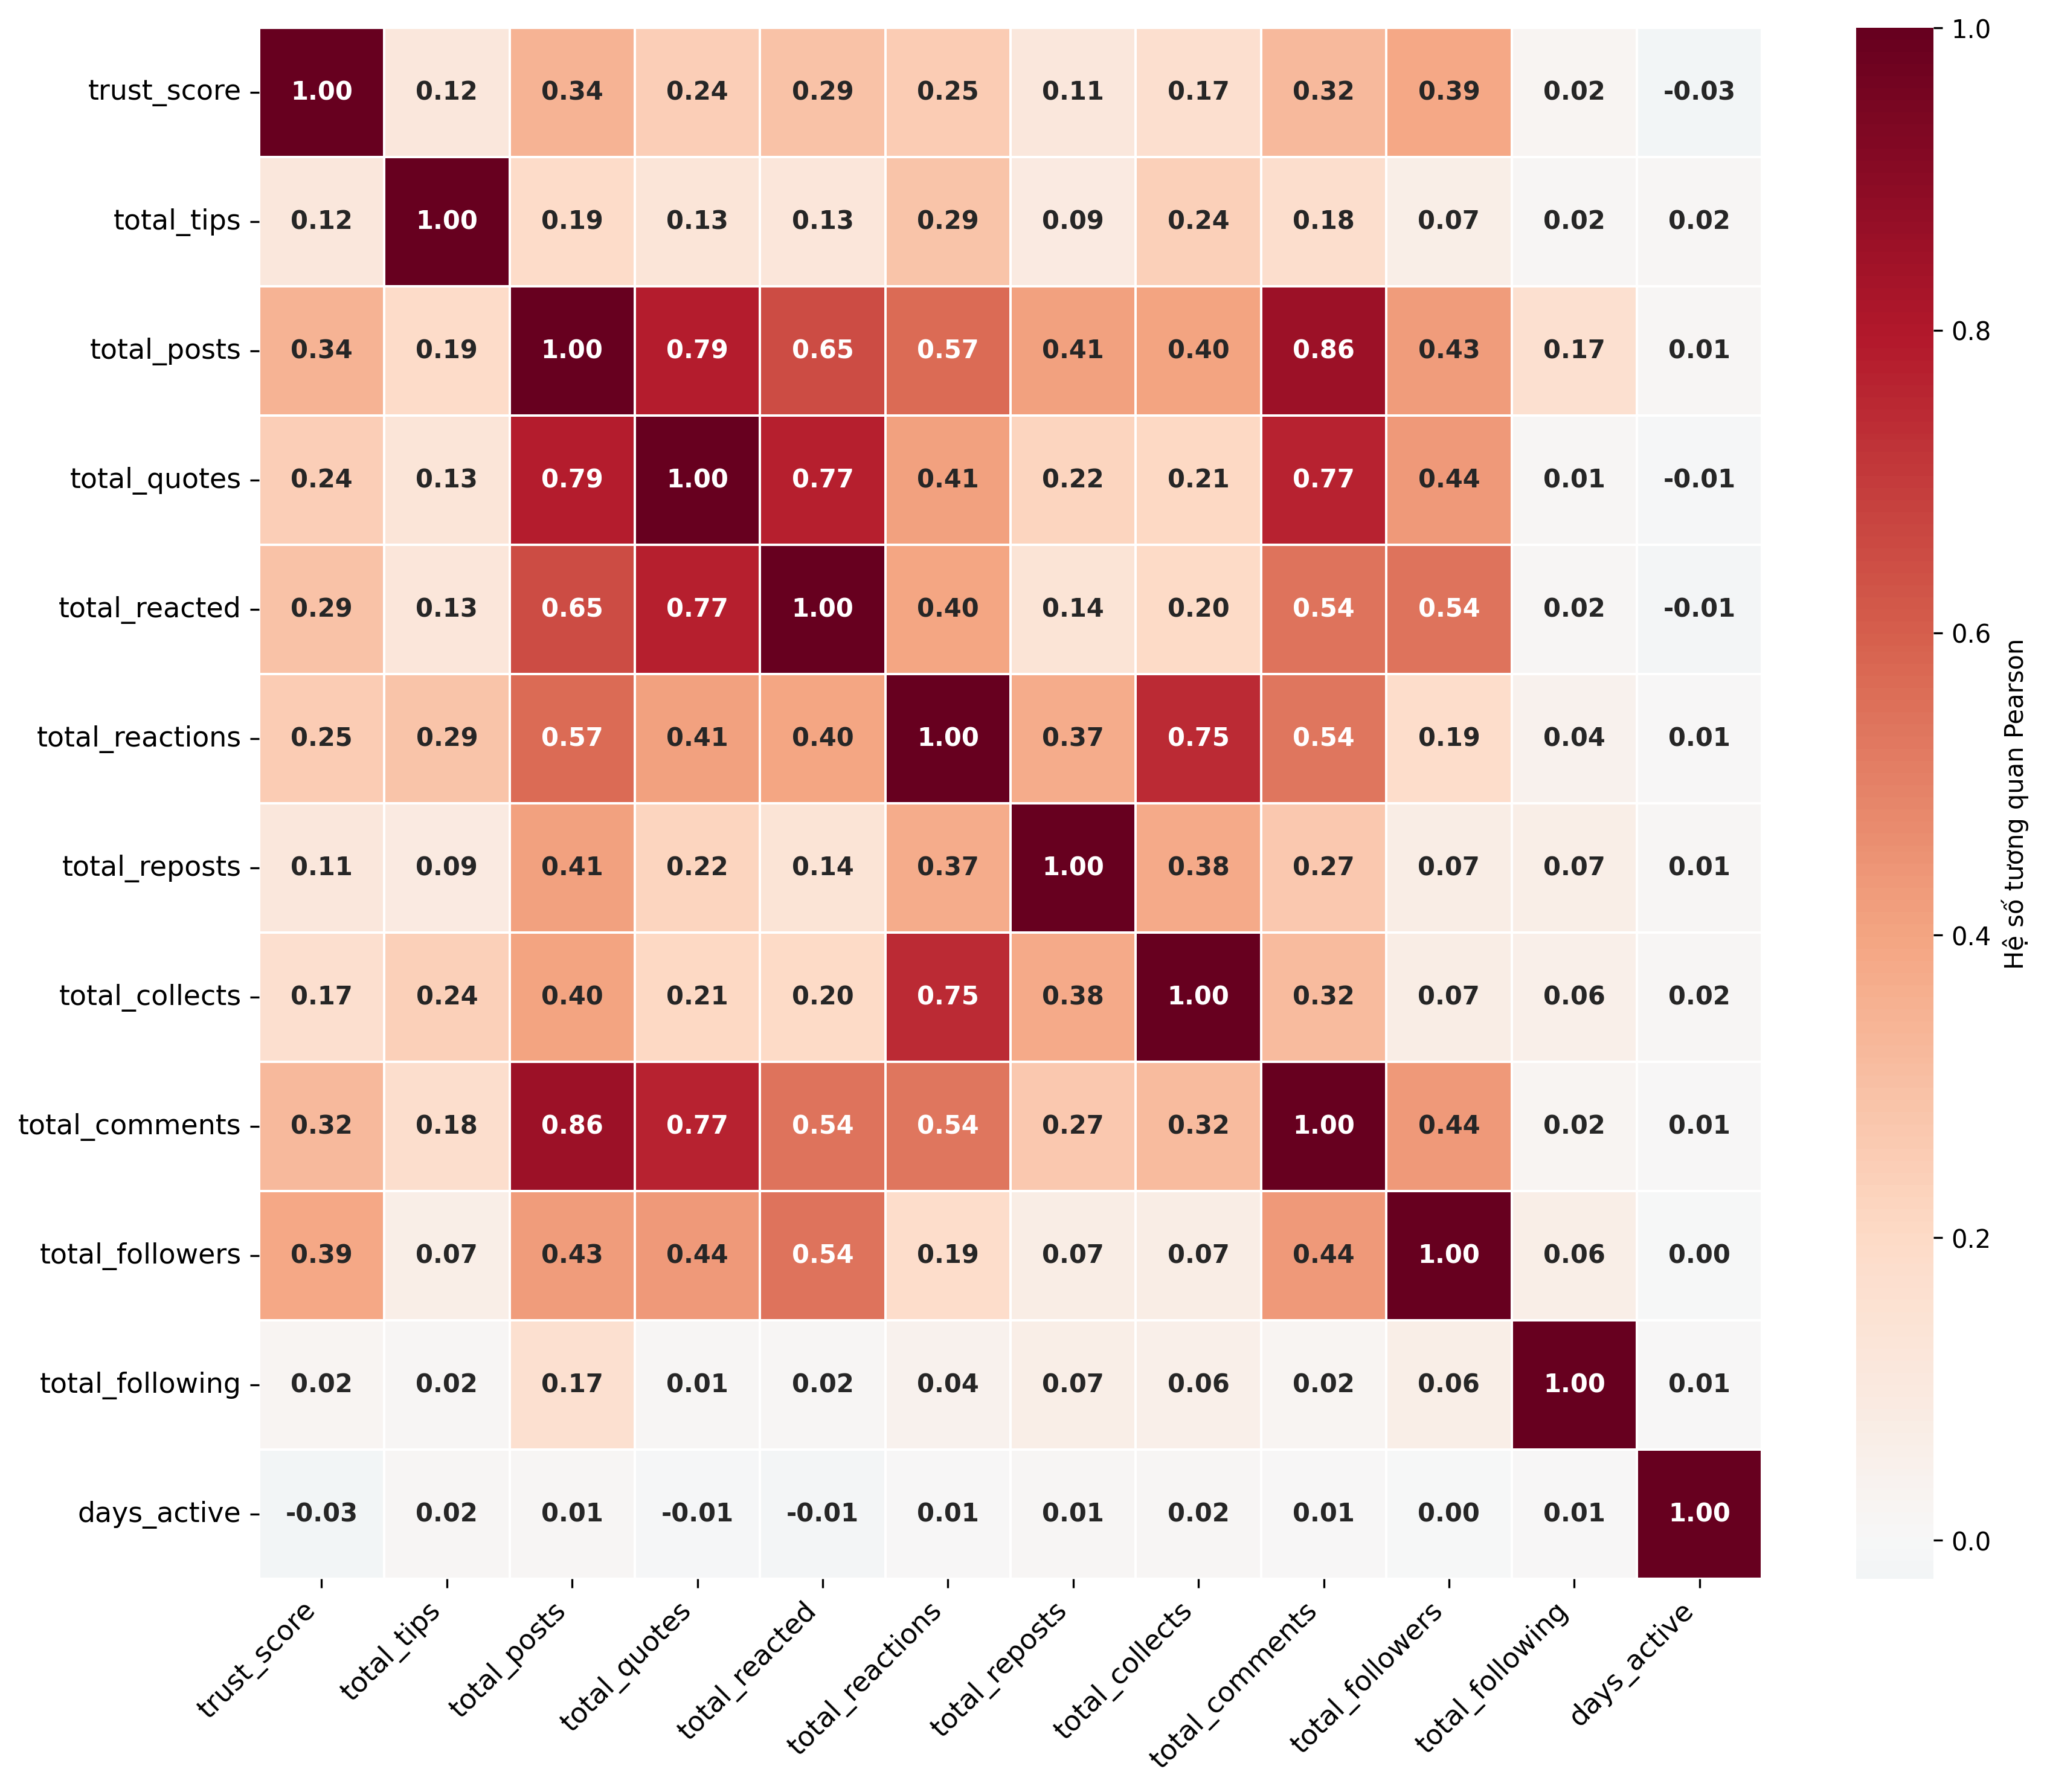
\includegraphics[width=\linewidth]{images/part-02/chap-02/sec-02/CorrelationHeatmapQuarter.png}
    \caption{Ma trận tương quan đặc trưng hành vi trên phạm vi dữ liệu Quý}
    \label{fig:FeatureCorrelation}
\end{figure}

Cuối cùng, vector đặc trưng của mỗi nút $v_i$ được hình thành thông qua phép ghép nối giữa vector ngữ nghĩa và vector hành vi:
\[
    X_i = [E_{semantic}(384) \parallel B_{behavioral}(12)] \in \mathbb{R}^{396}
\]
\indent Không gian đặc trưng \textbf{396 chiều} này đóng vai trò là dữ liệu đầu vào cho mô hình Graph Autoencoder và GNN baseline trong các quy trình gán nhãn giả lập và huấn luyện có giám sát ở các giai đoạn tiếp theo.\vspace{0.3cm}

%==========================================================================================

\textit{2.2.2. Chuẩn hóa trọng số liên kết đồ thị}\vspace{0.2cm}

\indent Trong các mạng xã hội phi tập trung như Lens Protocol, tần suất tương tác giữa các thực thể thường tuân theo quy luật lũy thừa. Thực tế cho thấy một số ít các liên kết sở hữu số lượng tương tác cực lớn, tạo nên sự mất cân bằng nghiêm trọng về mặt dữ liệu và mô hình GNN dễ gặp phải hiện tượng quá mịn.\vspace{0.3cm}

Để giải quyết vấn đề này, đề tài thực hiện chuẩn hóa trọng số cạnh thông qua hàm Logarithm nhằm nén biên độ của các liên kết quá mạnh nhưng vẫn bảo toàn được thứ tự ưu tiên của các tương tác. Trọng số cuối cùng của mỗi cạnh $e_{ij}$ được xác định theo công thức:

\[
    W_{final} = W_{base} \times \log(1 + \text{count})
\]

Trong đó, $W_{base}$ là trọng số cơ sở tương ứng với từng tầng quan hệ và \texttt{count} là tần suất tương tác thực tế.\vspace{0.3cm}

Hiệu quả của quy trình chuẩn hóa được minh chứng rõ rệt qua kết quả thực nghiệm tại \textbf{Hình \ref{fig:EdgeWeightDist}}. Trước khi xử lý, đồ thị tồn tại các cạnh có trọng số thô lên tới $2614.64$, gây nhiễu loạn cho các mô hình GNN quá trình học. Sau khi áp dụng hàm Logarithm, trọng số lớn nhất đã được nén xuống mức $69.69$, đưa toàn bộ các liên kết về một dải giá trị ổn định và đồng nhất hơn.

\begin{figure}[H]
    \centering
    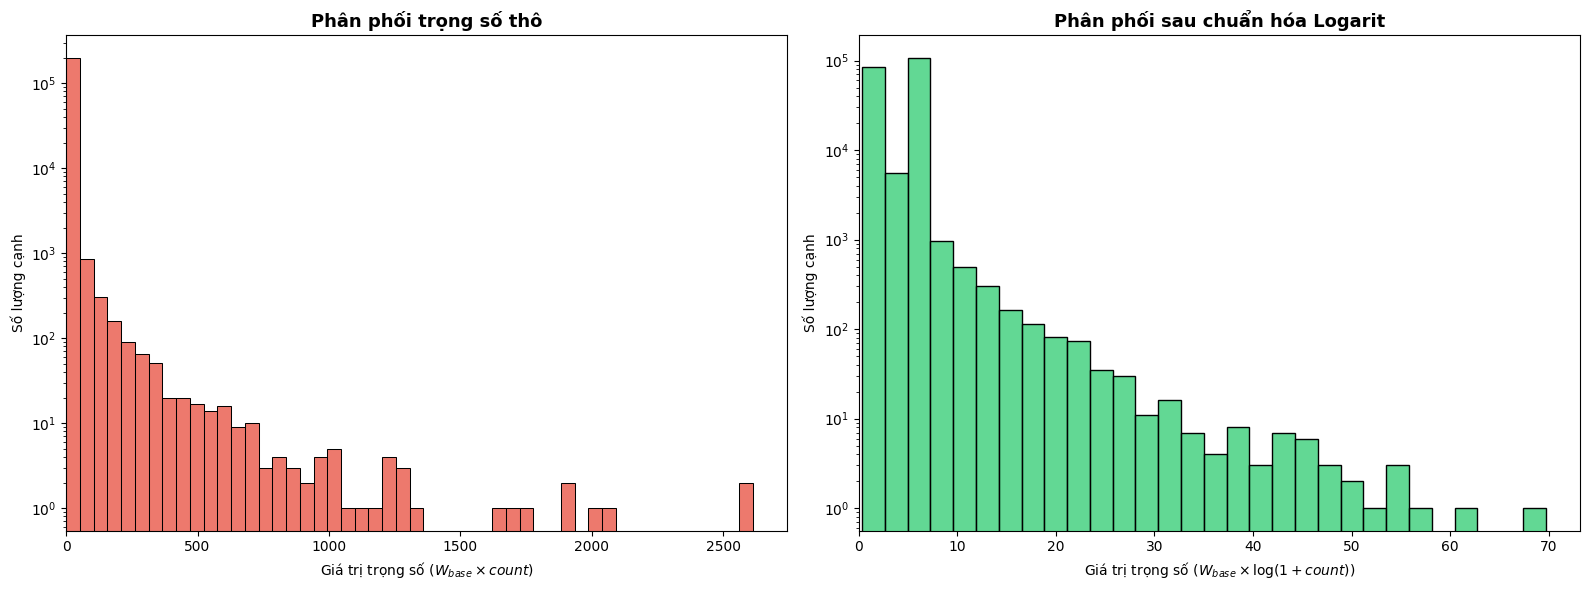
\includegraphics[width=1.0\linewidth]{images/part-02/chap-02/sec-02/EdgeWeightDistributionQuarter.png}
    \caption{So sánh phân phối trọng số cạnh trước và sau khi chuẩn hóa trên phạm vi Quý}
    \label{fig:EdgeWeightDist}
\end{figure}

Việc điều chỉnh này không chỉ giúp mô hình GNN hội tụ nhanh hơn mà còn đảm bảo tính khách quan trong việc tổng hợp đặc trưng từ các láng giềng đa tầng, từ đó nâng cao khả năng nhận diện các mô thức Sybil tinh vi trong mạng lưới.

% ==========================================================================================

\subsubsection{2.3. Xây dựng tập dữ liệu giám sát}

\indent\indent Do tính chất đặc thù của dữ liệu Web3 là thiếu hụt các nhãn thực tế, đề tài triển khai quy trình gán nhãn giả lập để xây dựng tập dữ liệu huấn luyện. Quy trình bắt đầu bằng việc sử dụng mô hình \textbf{Graph Autoencoder (GAE)} để nén không gian đặc trưng 396 chiều xuống không gian tiềm ẩn cấp thấp, qua đó bảo toàn cấu trúc liên kết đa tầng của đồ thị. Tiếp theo, thuật toán \textbf{K-Means} được áp dụng để gom cụm dựa trên sự tương đồng về vector embedding.\vspace{0.3cm}

Cuối cùng, các cụm hành vi này được ánh xạ và hợp nhất thành 04 loại nhãn chính dựa trên phân tích đặc tính trung bình của từng nhóm:
\begin{itemize}
    \item \textbf{Benign:} Tài khoản hoạt động tự nhiên, có điểm tin cậy cao và tương tác xã hội ổn định.
    \item \textbf{Low Risk:} Các tài khoản mới hoặc có tần suất hoạt động thấp nhưng chưa có dấu hiệu vi phạm.
    \item \textbf{High Risk:} Nhóm có hành vi tương tác bất thường, tần suất cao trong thời gian ngắn, tiềm ẩn rủi ro spam.
    \item \textbf{Malicious:} Các nút có sự tương đồng cực cao về tiểu sử và cấu trúc liên kết đồng sở hữu, đặc trưng của mạng lưới Sybil chuyên nghiệp.
\end{itemize}

\begin{figure}[H]
    \centering
    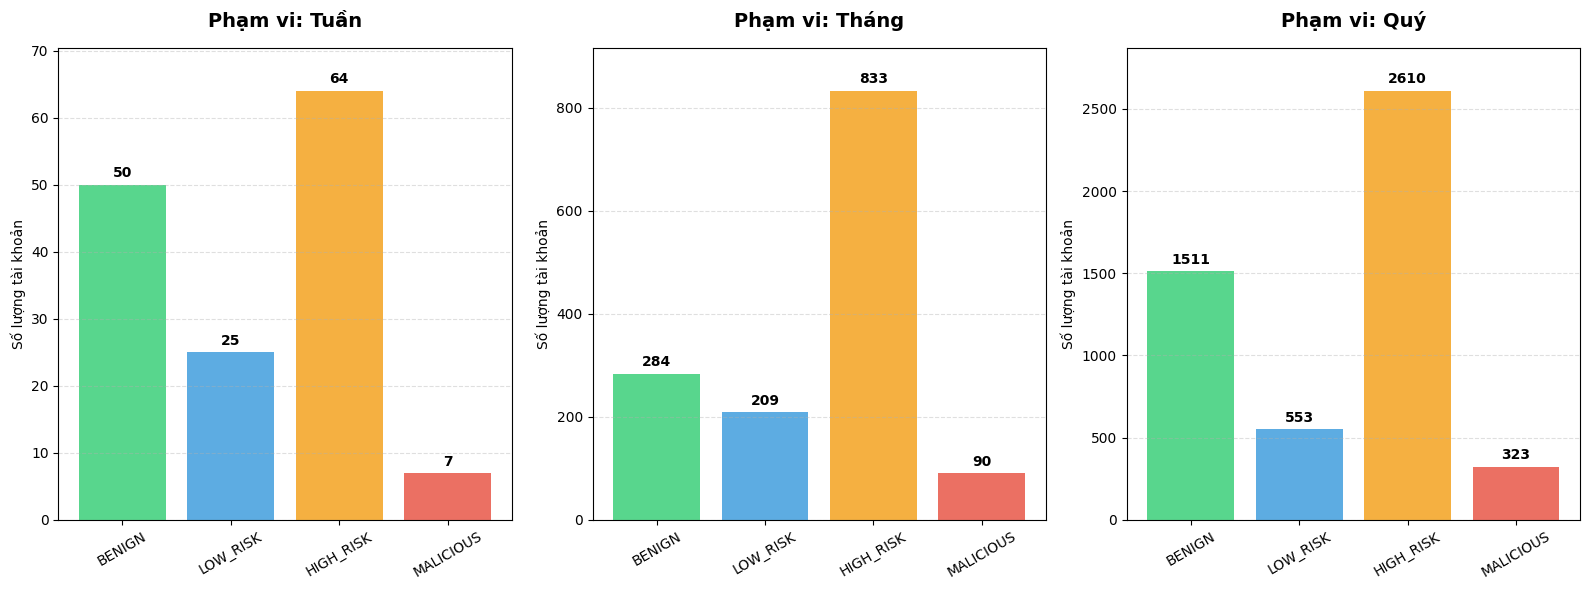
\includegraphics[width=\linewidth]{images/part-02/chap-02/sec-02/LabelDistributionComparison.png}
    \caption{Phân bổ nhãn giả lập qua các phạm vi thời gian thực nghiệm}
    \label{fig:LabelDist}
\end{figure}

Kết quả phân bổ tại \textbf{Hình \ref{fig:LabelDist}} cho thấy quy mô của các nhóm nhãn tăng trưởng tỉ lệ thuận với phạm vi thời gian thu thập. Đáng chú ý, số lượng nhãn \textbf{Malicious} tăng mạnh từ 7 thực thể (phạm vi Tuần) lên 323 thực thể (phạm vi Quý). Điều này chứng minh rằng các mô thức tấn công Sybil có xu hướng lộ diện rõ nét hơn khi quan sát trên cấu trúc đồ thị ổn định dài hạn, nơi các mối quan hệ đa tầng được thiết lập đủ dày đặc để thực hiện các thuật toán phân tách hành vi.

% ==========================================================================================

\subsubsection{2.4. Chiến lược cân bằng và chia tập dữ liệu}

\indent\indent Để đảm bảo tính khách quan và tối ưu hóa khả năng hội tụ của các mô hình, đề tài thực hiện thiết lập trọng số lớp và phân chia dữ liệu một cách hệ thống trên cả ba phạm vi thời gian nghiên cứu.\vspace{0.3cm}

\textit{2.4.1. Xử lý mất cân bằng nhãn}\vspace{0.2cm}

Sự chênh lệch đáng kể về số lượng giữa các lớp hành vi — đặc biệt là sự thiểu số của lớp \textit{Malicious}. Để khắc phục, đề tài áp dụng sử dụng trọng số lớp trong hàm mất mát. Trọng số được tính toán nghịch đảo với tần suất xuất hiện của mỗi lớp trong tập huấn luyện, buộc mô hình phải tăng cường sự tập trung vào các nhóm thực thể rủi ro cao.\vspace{0.3cm}

Chi tiết các giá trị trọng số được áp dụng cho từng phạm vi dữ liệu được trình bày tại \textbf{Bảng \ref{tab:ClassWeights}}. Có thể thấy tại phạm vi Quý, lớp \textit{Malicious} được gán trọng số $3.8634$, cao hơn gấp 8 lần so với lớp \textit{High Risk} ($0.4786$), giúp đảm bảo độ nhạy trong việc nhận diện Sybil.

\begin{table}[H]
    \centering
    \caption{Trọng số lớp (Class Weights) tính toán trên tập huấn luyện}
    \label{tab:ClassWeights}
    \setlength{\tabcolsep}{8pt}
    \renewcommand{\arraystretch}{1.2}
    \begin{tabular}{|l|c|c|c|c|}
        \hline
        \textbf{Phạm vi} & \textbf{BENIGN} & \textbf{LOW\_RISK} & \textbf{HIGH\_RISK} & \textbf{MALICIOUS} \\ \hline
        Tuần  & 0.7250 & 1.4500 & 0.5724 & 5.4375 \\ \hline
        Tháng & 1.2485 & 1.6980 & 0.4245 & 3.9306 \\ \hline
        Quý   & 0.8273 & 2.2575 & 0.4786 & 3.8634 \\ \hline
    \end{tabular}
\end{table}

\textit{2.4.2. Phân chia tập dữ liệu}\vspace{0.2cm}

Toàn bộ các thực thể trong mỗi phạm vi nghiên cứu được phân chia theo tỷ lệ cố định: 60\% dành cho huấn luyện (\textit{Train}), 20\% cho đánh giá (\textit{Validation}) và 20\% cho kiểm thử (\textit{Test}). Dữ liệu thực nghiệm tại phạm vi Quý ghi nhận quy mô lớn nhất với 2998 nút huấn luyện và 1000 nút kiểm thử, tạo điều kiện thuận lợi cho việc kiểm chứng khả năng tổng quát hóa của hệ thống trên dữ liệu thực tế quy mô lớn. Chi tiết phân bổ quy mô dữ liệu qua các phạm vi được tổng hợp tại \textbf{Bảng \ref{tab:DataSplitSize}}.

\begin{table}[H]
    \centering
    \caption{Quy mô phân chia tập dữ liệu qua các phạm vi thực nghiệm}
    \label{tab:DataSplitSize}
    \setlength{\tabcolsep}{12pt}
    \renewcommand{\arraystretch}{1.2}
    \begin{tabular}{|l|c|c|c|c|}
        \hline
        \textbf{Phạm vi} & \textbf{Train (60\%)} & \textbf{Val (20\%)} & \textbf{Test (20\%)} & \textbf{Tổng số} \\ \hline
        Tuần  & 87   & 29  & 30   & 146  \\ \hline
        Tháng & 849  & 283 & 284  & 1416 \\ \hline
        Quý   & 2998 & 999 & 1000 & 4997 \\ \hline
    \end{tabular}
\end{table}